%%%%%%%%%%%%%%%%%%%%%%%%%%%%%%%%%%%%%%%%%
% Beamer Presentation
% LaTeX Template
% Version 1.0 (10/11/12)
%
% This template has been downloaded from:
% http://www.LaTeXTemplates.com
%
% License:
% CC BY-NC-SA 3.0 (http://creativecommons.org/licenses/by-nc-sa/3.0/)
%
%%%%%%%%%%%%%%%%%%%%%%%%%%%%%%%%%%%%%%%%%

%----------------------------------------------------------------------------------------
%	PACKAGES AND THEMES
%----------------------------------------------------------------------------------------

\documentclass{beamer}

\mode<presentation> {

% The Beamer class comes with a number of default slide themes
% which change the colors and layouts of slides. Below this is a list
% of all the themes, uncomment each in turn to see what they look like.

%\usetheme{default}
%\usetheme{AnnArbor}
%\usetheme{Antibes}
%\usetheme{Bergen}
%\usetheme{Berkeley}
%\usetheme{Berlin}
%\usetheme{Boadilla}
%\usetheme{CambridgeUS}
%\usetheme{Copenhagen}
%\usetheme{Darmstadt}
%\usetheme{Dresden}
%\usetheme{Frankfurt}
%\usetheme{Goettingen}
%\usetheme{Hannover}
%\usetheme{Ilmenau}
%\usetheme{JuanLesPins}
%\usetheme{Luebeck}
\usetheme{Madrid}
%\usetheme{Malmoe}
%\usetheme{Marburg}
%\usetheme{Montpellier}
%\usetheme{PaloAlto}
%\usetheme{Pittsburgh}
%\usetheme{Rochester}
%\usetheme{Singapore}
%\usetheme{Szeged}
%\usetheme{Warsaw}

% As well as themes, the Beamer class has a number of color themes
% for any slide theme. Uncomment each of these in turn to see how it
% changes the colors of your current slide theme.

%\usecolortheme{albatross}
%\usecolortheme{beaver}
%\usecolortheme{beetle}
%\usecolortheme{crane}
%\usecolortheme{dolphin}
%\usecolortheme{dove}
%\usecolortheme{fly}
%\usecolortheme{lily}
%\usecolortheme{orchid}
%\usecolortheme{rose}
%\usecolortheme{seagull}
%\usecolortheme{seahorse}
%\usecolortheme{whale}
%\usecolortheme{wolverine}

%\setbeamertemplate{footline} % To remove the footer line in all slides uncomment this line
%\setbeamertemplate{footline}[page number] % To replace the footer line in all slides with a simple slide count uncomment this line

%\setbeamertemplate{navigation symbols}{} % To remove the navigation symbols from the bottom of all slides uncomment this line
}
\usepackage[T1]{fontenc}

\usepackage{graphicx} % Allows including images
\usepackage{booktabs} % Allows the use of \toprule, \midrule and \bottomrule in tables
\usepackage{array,multirow,graphicx}
\usepackage{todonotes}
\newcommand{\todosk}[1]{\todo[inline]{#1}} 
\usepackage{media9} 
\usepackage{listings} % Required for insertion of code
\usepackage{courier} % Required for the courier font
\usepackage{listings}
\usepackage{color}
\usepackage{hyperref}
\usepackage{verbatim}
\usepackage[autostyle]{csquotes}


\definecolor{dkgreen}{rgb}{0,0.6,0}
\definecolor{gray}{rgb}{0.5,0.5,0.5}
\definecolor{mauve}{rgb}{0.58,0,0.82}

\lstset{frame=tb,
  language=Bash,
  aboveskip=3mm,
  belowskip=3mm,
  showstringspaces=false,
  columns=flexible,
  basicstyle={\small\ttfamily},
  numbers=none,
  numberstyle=\tiny\color{gray},
  keywordstyle=\color{blue},
  commentstyle=\color{dkgreen},
  stringstyle=\color{mauve},
  breaklines=true,
  breakatwhitespace=true
  tabsize=3
}


%----------------------------------------------------------------------------------------
%	TITLE PAGE
%----------------------------------------------------------------------------------------

\title[Git Guide]{Git Guide} % The short title appears at the bottom of every slide, the full title is only on the title page

\author{Sr\dj{}an Krsti\'c, Claudio Menghi} % Your name
\institute[] % Your institution as it will appear on the bottom of every slide, may be shorthand to save space
{
Politecnico di Milano \\ % Your institution for the title page
\medskip
\textit{srdan.krstic@polimi.it, claudio.menghi@polimi.it} % Your email address
}
\date{\today} % Date, can be changed to a custom date




\begin{document}

\begin{frame}
\titlepage % Print the title page as the first slide
\end{frame}


%----------------------------------------------------------------------------------------
%	PRESENTATION SLIDES
%----------------------------------------------------------------------------------------



\section{Overview}
\begin{frame}
\frametitle{Overview}


\begin{itemize}
\item Introduction
\item Using Git locally
  \begin{itemize}
  \item git configure
  \item git init
  \item git status
  \item git add
  \item git commit
  \item git log
  \item git branch
  \item git checkout
  \item git merge
  \end{itemize}
\item Using Git remotely
  \begin{itemize}
  \item git clone
  \item git remote
  \item git fetch
  \item git pull
  \item git push
  \end{itemize}
\item Using Git with Eclipse
\end{itemize}
\end{frame}


% {
% %\usebackgroundtemplate{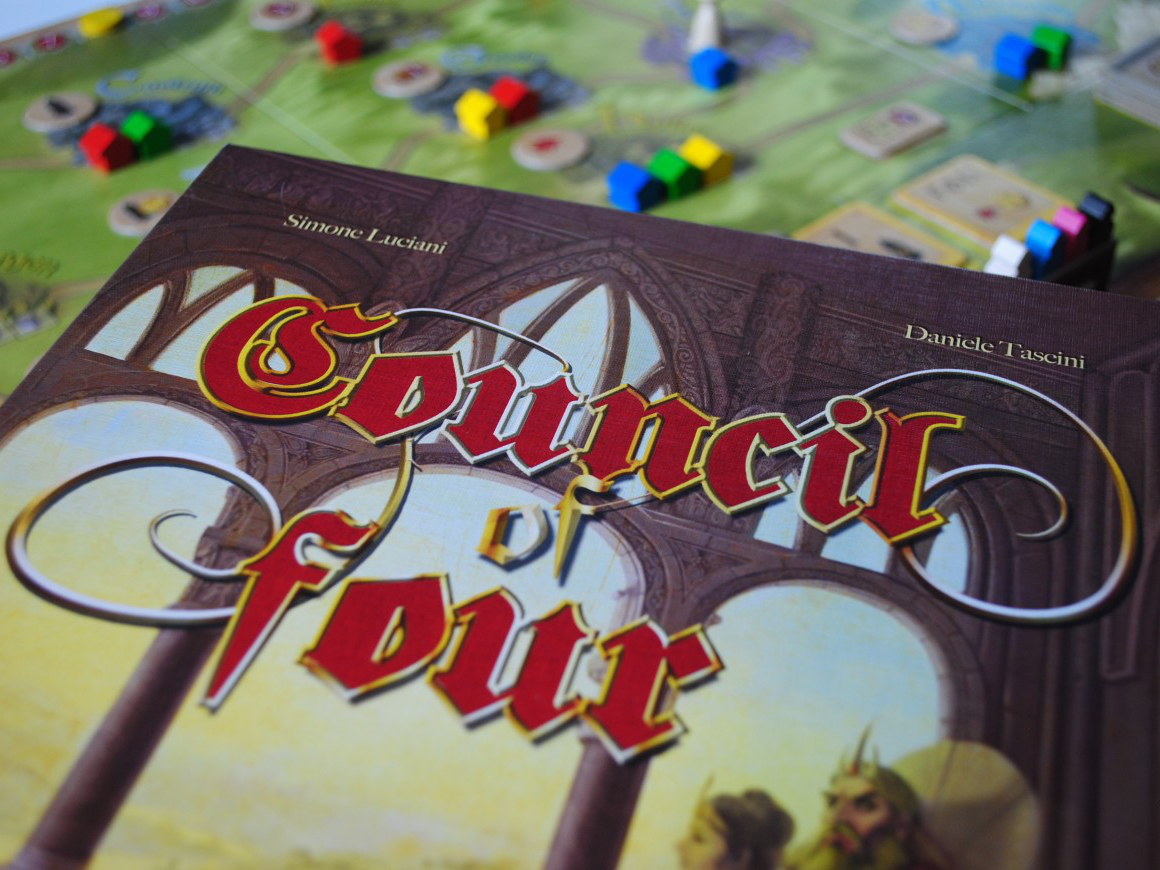
\includegraphics[width=\paperwidth]{cover1.jpg}}%
% \begin{frame}[plain]


% \end{frame}
% }

\begin{frame}

\LARGE	
\textbf{Introduction}


\end{frame}

\section{Introduction}
\begin{frame}
\frametitle{What is a version control system (VCS)?}


A version control system is a piece of software that helps the
developers to \textbf{collaborate} remotely and to \textbf{keep track} of the
history of their work. 

\end{frame}


\begin{frame}
\frametitle{Goals of VCS}

\begin{itemize}
\item enable simultaneous work
\item easily resolve conflicts
\item keep the history
\item also, to do all this fast and error-free
\end{itemize}
\end{frame}



\begin{frame}
\frametitle{First generation VCS}
Local versioning + Exchanging patches

\begin{figure}


\includegraphics[scale=0.3]{figures/f4.png}

\includegraphics[scale=0.3]{figures/f3.png}
\end{figure}

\end{frame}

\begin{frame}
\frametitle{Second generation VCS}
Remote centralized versioning


\begin{figure}
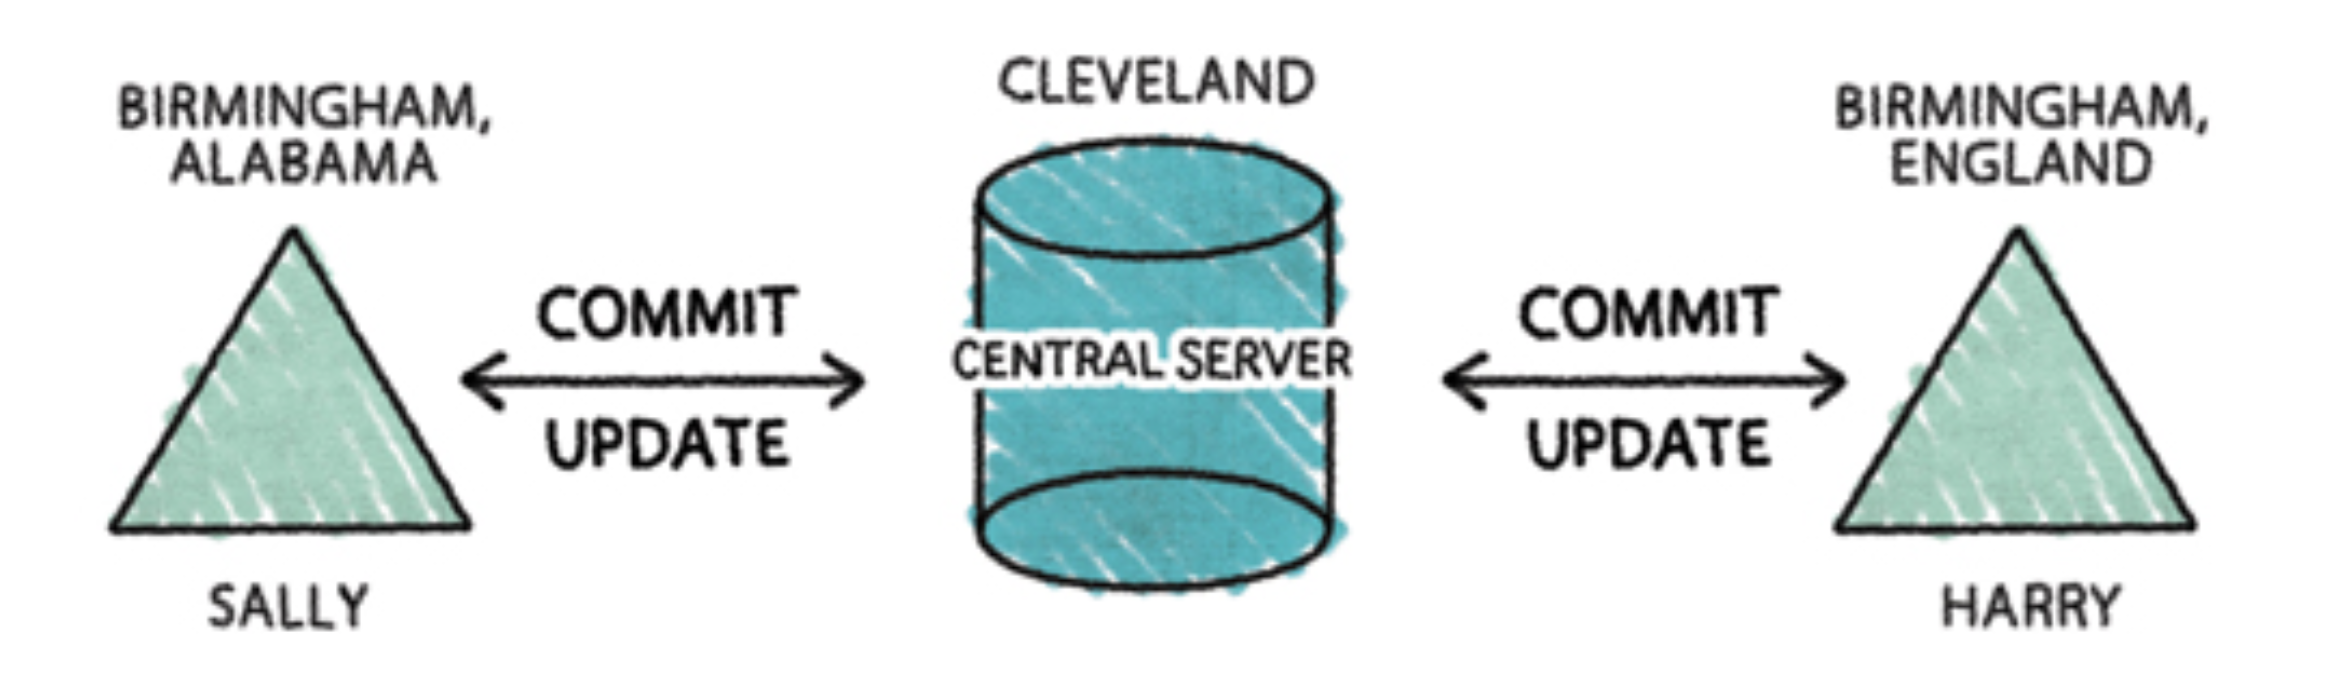
\includegraphics[scale=0.3]{figures/f1.png}
\end{figure}


\end{frame}

\begin{frame}
\frametitle{Third generation VCS}
Remote distributed versioning


\begin{figure}
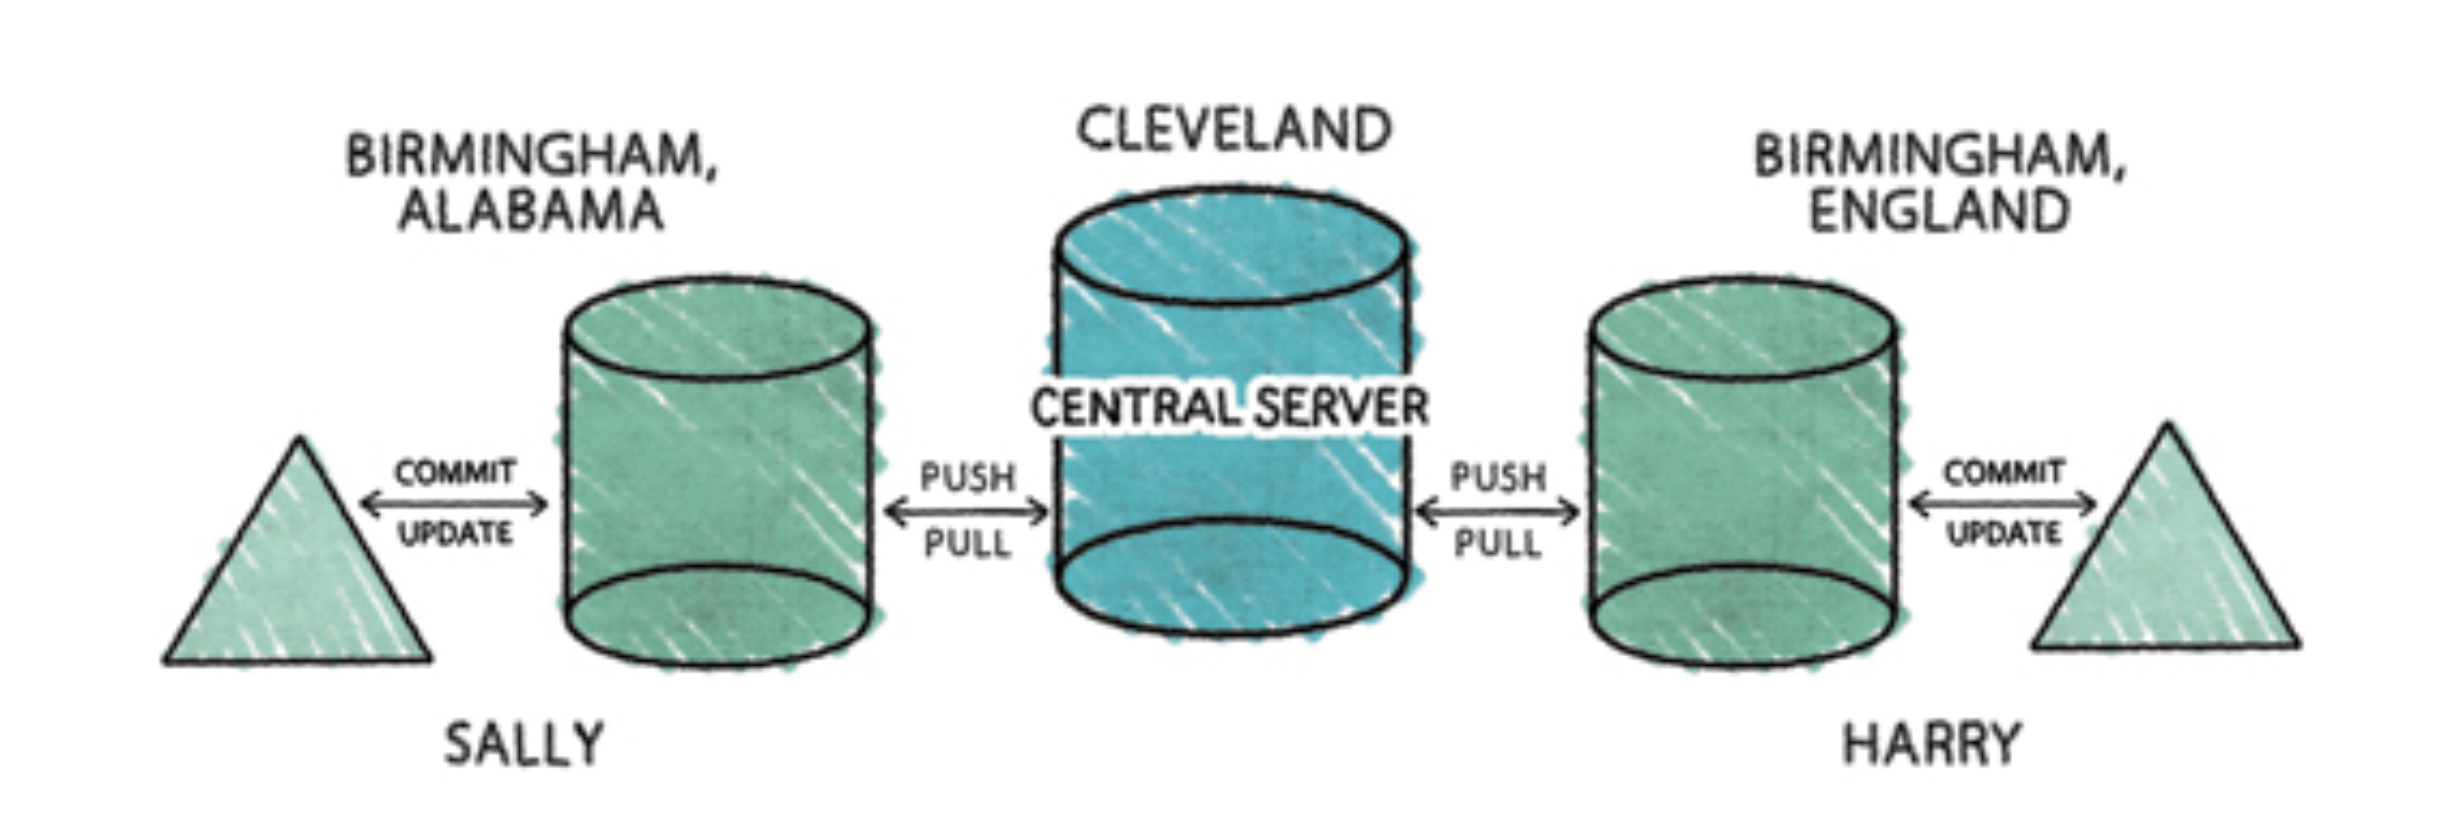
\includegraphics[scale=0.28]{figures/f2.png}
\end{figure}

\end{frame}


\begin{frame}

\LARGE	
\textbf{Using Git locally}


\end{frame}


\begin{frame}
\frametitle{Creating a Git repository}

\begin{itemize}
\item Creating an empty repository 
\item ``Cloning'' an existing repository (see Using Git remotely)
\end{itemize}

\end{frame}


\begin{frame}[fragile]
\frametitle{git init}
Creating a repository in folder "testrepo''
\begin{lstlisting}
$ git init testrepo
$ tree -a
|-- .git
    |-- HEAD
    |-- config
    |-- description
    |-- hooks
    |-- info
    |   |-- exclude
    |-- objects
    |   |-- info
    |   |-- pack
    |-- refs
        |-- heads
        |-- tags
9 directories, 13 files
\end{lstlisting}

\end{frame}


\begin{frame}
\frametitle{Edit-Stage-Commit workflow}
~~~~~~~~Untracked files~~~~~~~~~~~~~~~Staged files~~~~~~~~~~~~Committed files
\begin{figure}
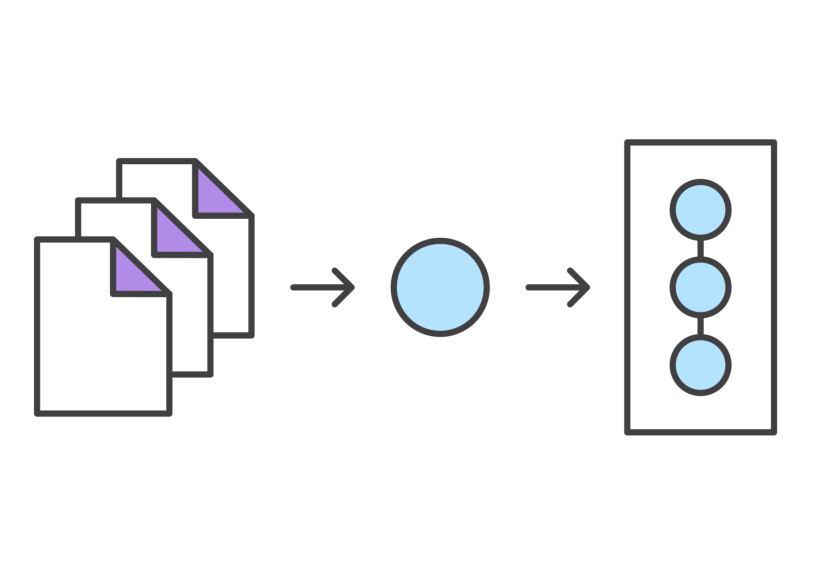
\includegraphics[scale=0.7]{figures/04.pdf}
\end{figure}

\end{frame}

\begin{frame}[fragile]
\frametitle{git add}

Staging files to be saved in the repository

\begin{lstlisting}
$ touch Main.java
$ git add Main.java
\end{lstlisting}

\end{frame}


\begin{frame}[fragile]
\frametitle{git status}

Checking the status of the working folder.

\begin{lstlisting}
$ git status
$ git touch Test.java
$ git status
$ git add Test.java
\end{lstlisting}
\end{frame}


\begin{frame}[fragile]
\frametitle{git commit}

Writing to the local repository

\begin{lstlisting}
$ git commit -m "First commit"
$ git status
\end{lstlisting}
\end{frame}


\begin{frame}
\frametitle{First commit}
First commit
\begin{figure}

\includegraphics[scale=0.4]{figures/f8.png}
\end{figure}

\end{frame}


\begin{frame}
\frametitle{Commit representation}

\begin{figure}

\includegraphics[scale=0.3]{figures/f9.png}
\end{figure}

\end{frame}



\begin{frame}[fragile]
\frametitle{More commits}

Perform some more commits...

\begin{lstlisting}
# some modifications
$ git commit -m "Second commit"
$ git status
\end{lstlisting}
\end{frame}


\begin{frame}[fragile]
\frametitle{git log}

\begin{lstlisting}
$ git log
$ git log --online
\end{lstlisting}
\end{frame}

\begin{frame}[fragile]
\frametitle{Hands on - Committing (5 mins)}

Execute these commands:

\begin{lstlisting}
$ git init testrepo
$ git status
$ # create some files
$ git status
$ git add <some files>
$ git status
$ git commit -m "<message>"
$ git status
$ git log
$ # create some more commits
$ git log
$
\end{lstlisting}
\end{frame}



\begin{frame}
\frametitle{Changes as a directed acyclic graph (DAG)}

\begin{figure}
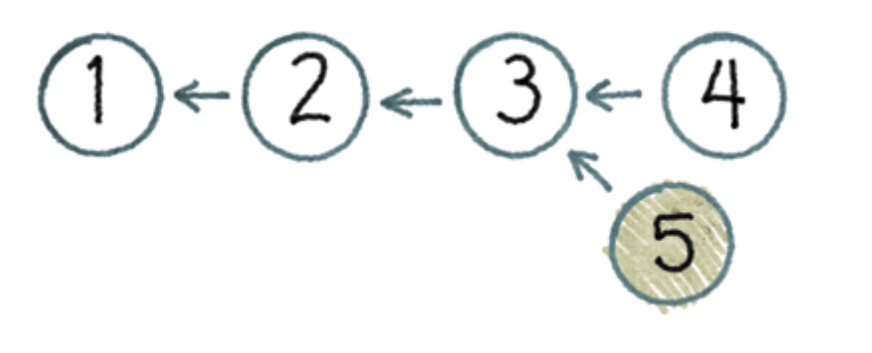
\includegraphics[scale=0.3]{figures/f10.png}
\end{figure}

\end{frame}

\begin{frame}
\frametitle{Changes as a directed acyclic graph (DAG)}

\begin{figure}
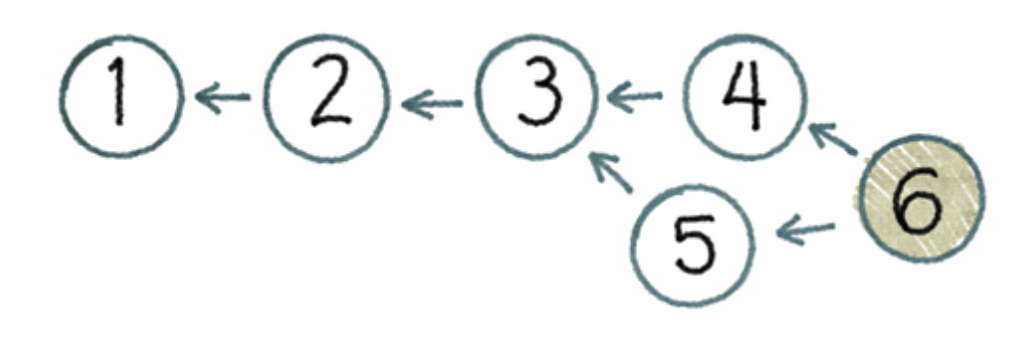
\includegraphics[scale=0.3]{figures/f11.png}
\end{figure}

\end{frame}


\begin{frame}
\frametitle{Changes as a directed acyclic graph (DAG)}

\begin{figure}
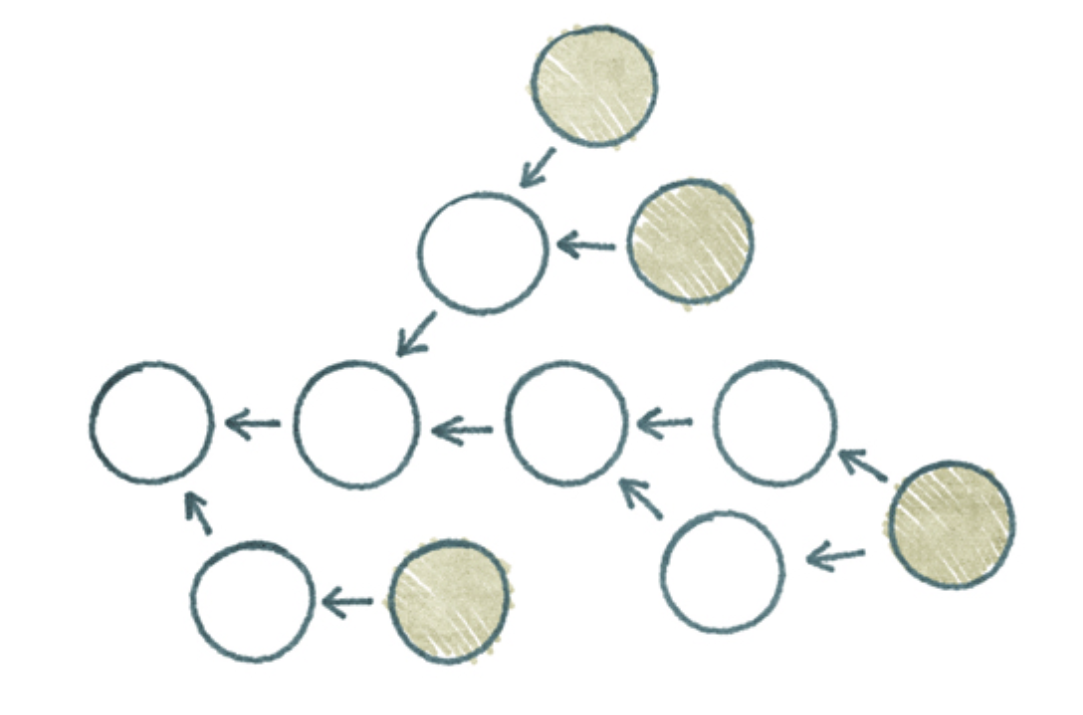
\includegraphics[scale=0.3]{figures/f12.png}
\end{figure}

\end{frame}


\begin{frame}[fragile]
\frametitle{git branch}

Creating and modifying branches

\begin{lstlisting}
$ git branch feature 
$ git branch -m feature-GUI-Swing
$ git branch 
$
\end{lstlisting}
\end{frame}


\begin{frame}[fragile]
\frametitle{git checkout}

Changing between branches

\begin{lstlisting}
$ git checkout feature-GUI-Swing
$ touch GUI.java
$ # try to switch between the branches
$ git add GUI.java
$ # try to switch between the branches
$ git commit -m  "added gui"
$ # try to switch between the branches
$ git log --graph --oneline --decorate
\end{lstlisting}
\end{frame}


\begin{frame}
\frametitle{Merging branches (fast-forward merge)}

\begin{figure}
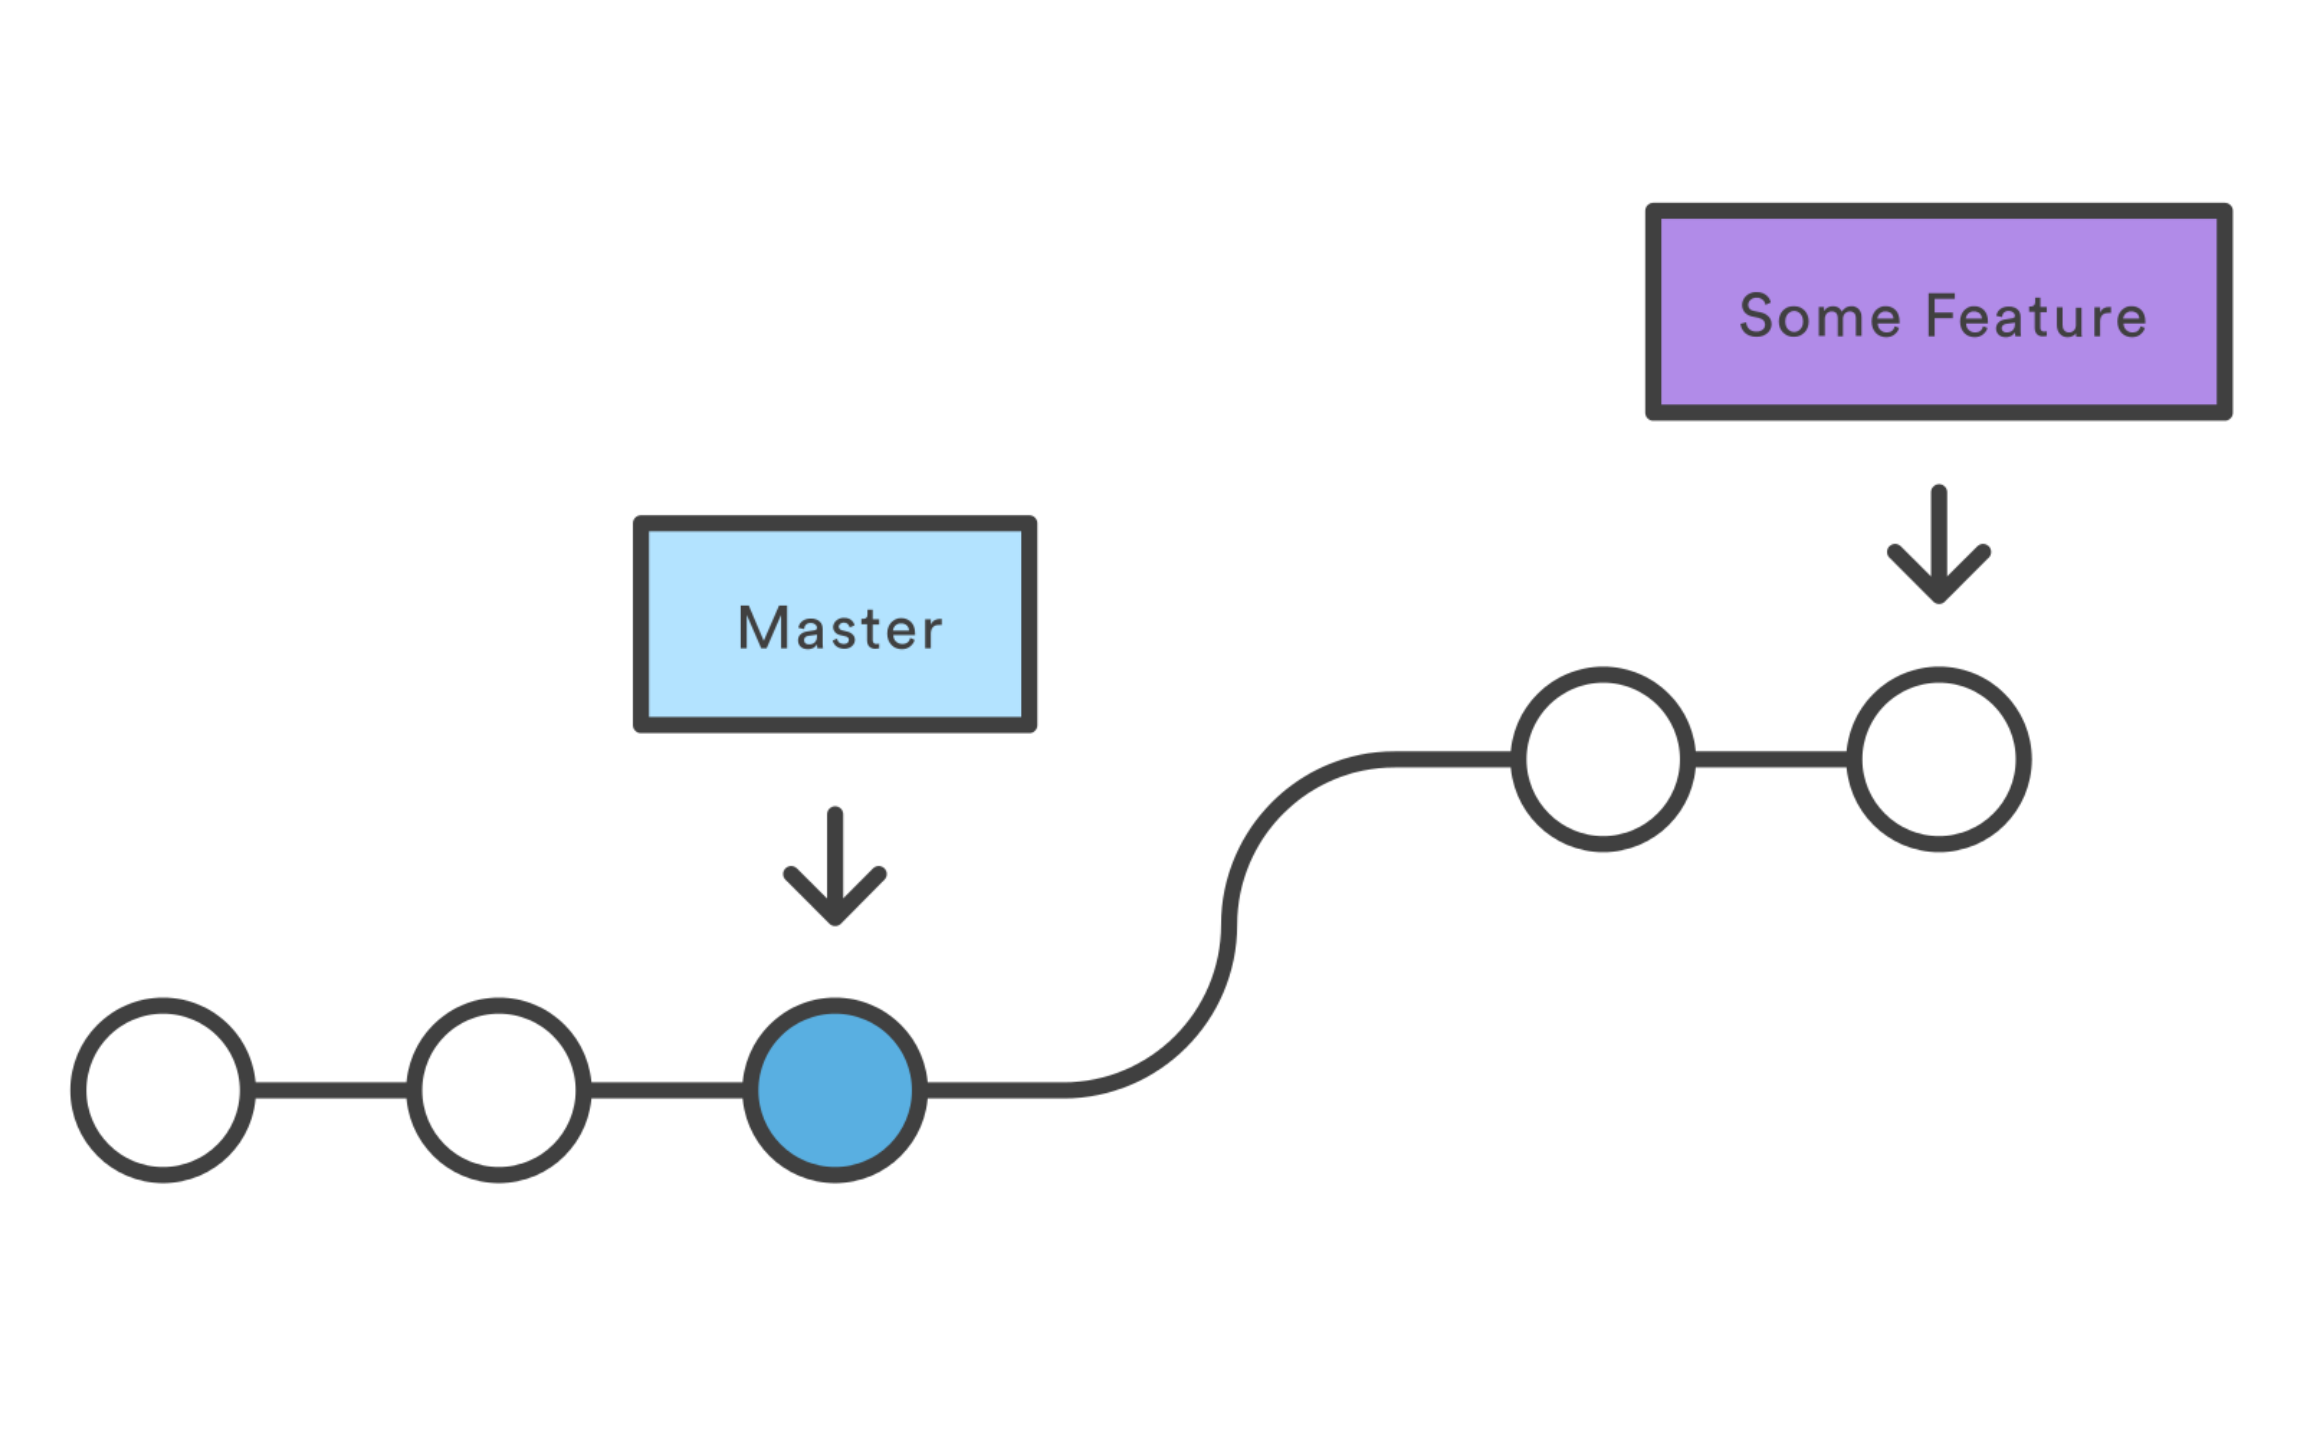
\includegraphics[scale=0.8]{figures/f13.png}
\end{figure}

\end{frame}

\begin{frame}
\frametitle{Merging branches (fast-forward merge)}

\begin{figure}
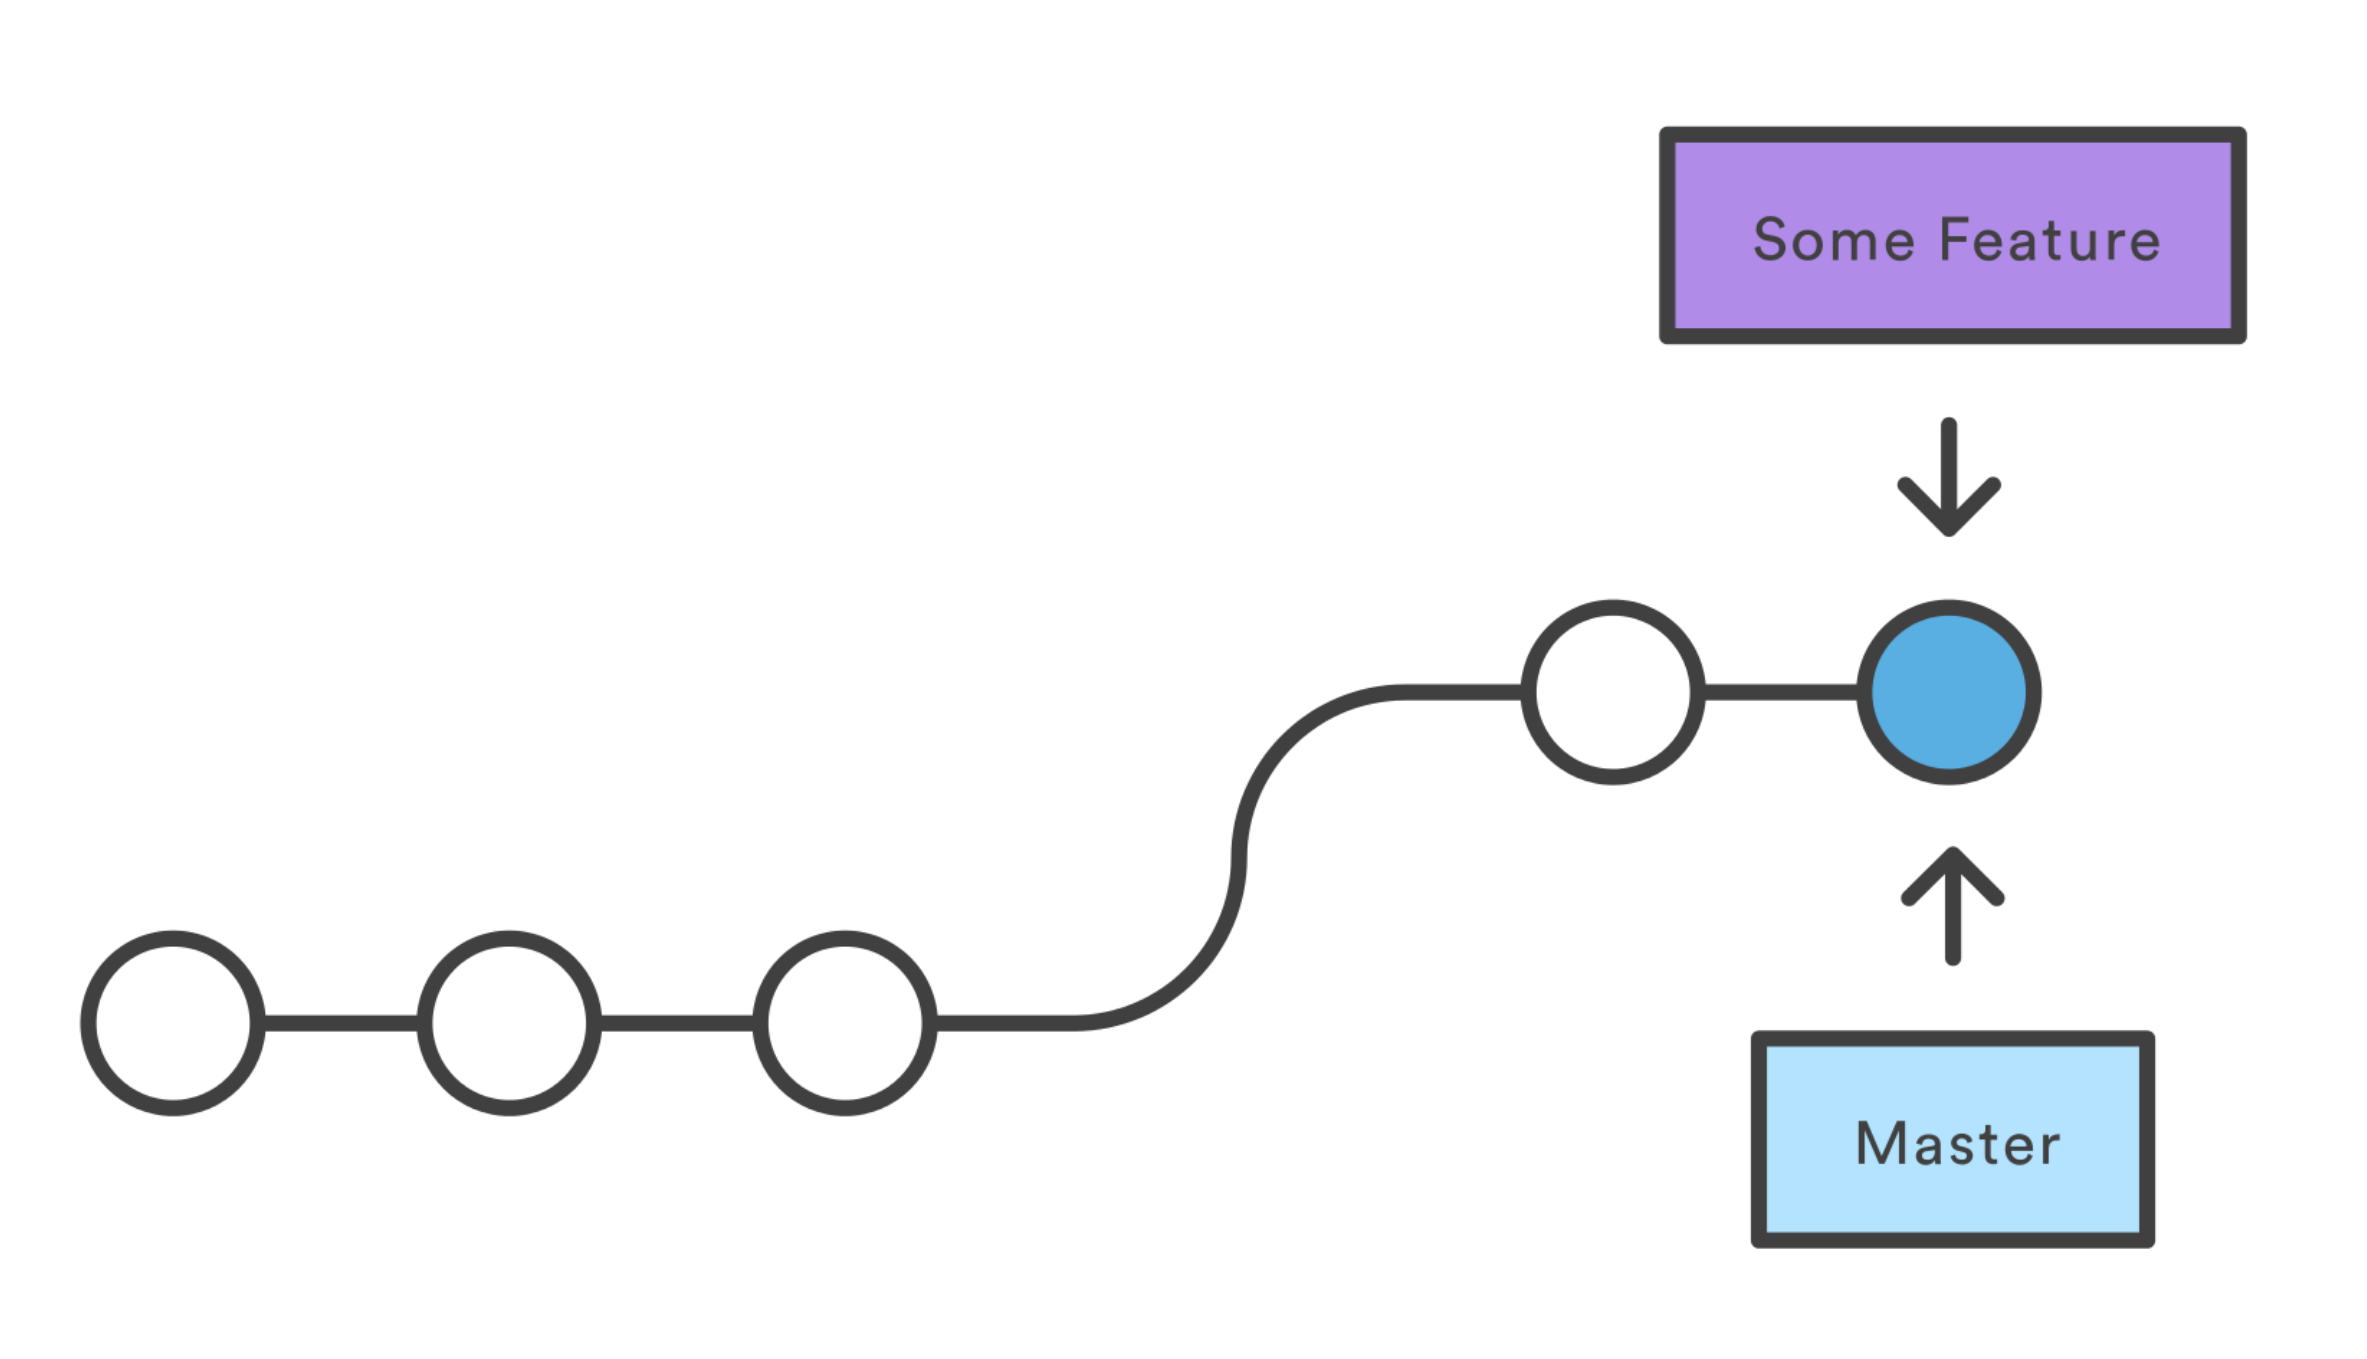
\includegraphics[scale=0.8]{figures/f14.png}
\end{figure}

\end{frame}


\begin{frame}
\frametitle{Merging branches (3-way merge)}

\begin{figure}
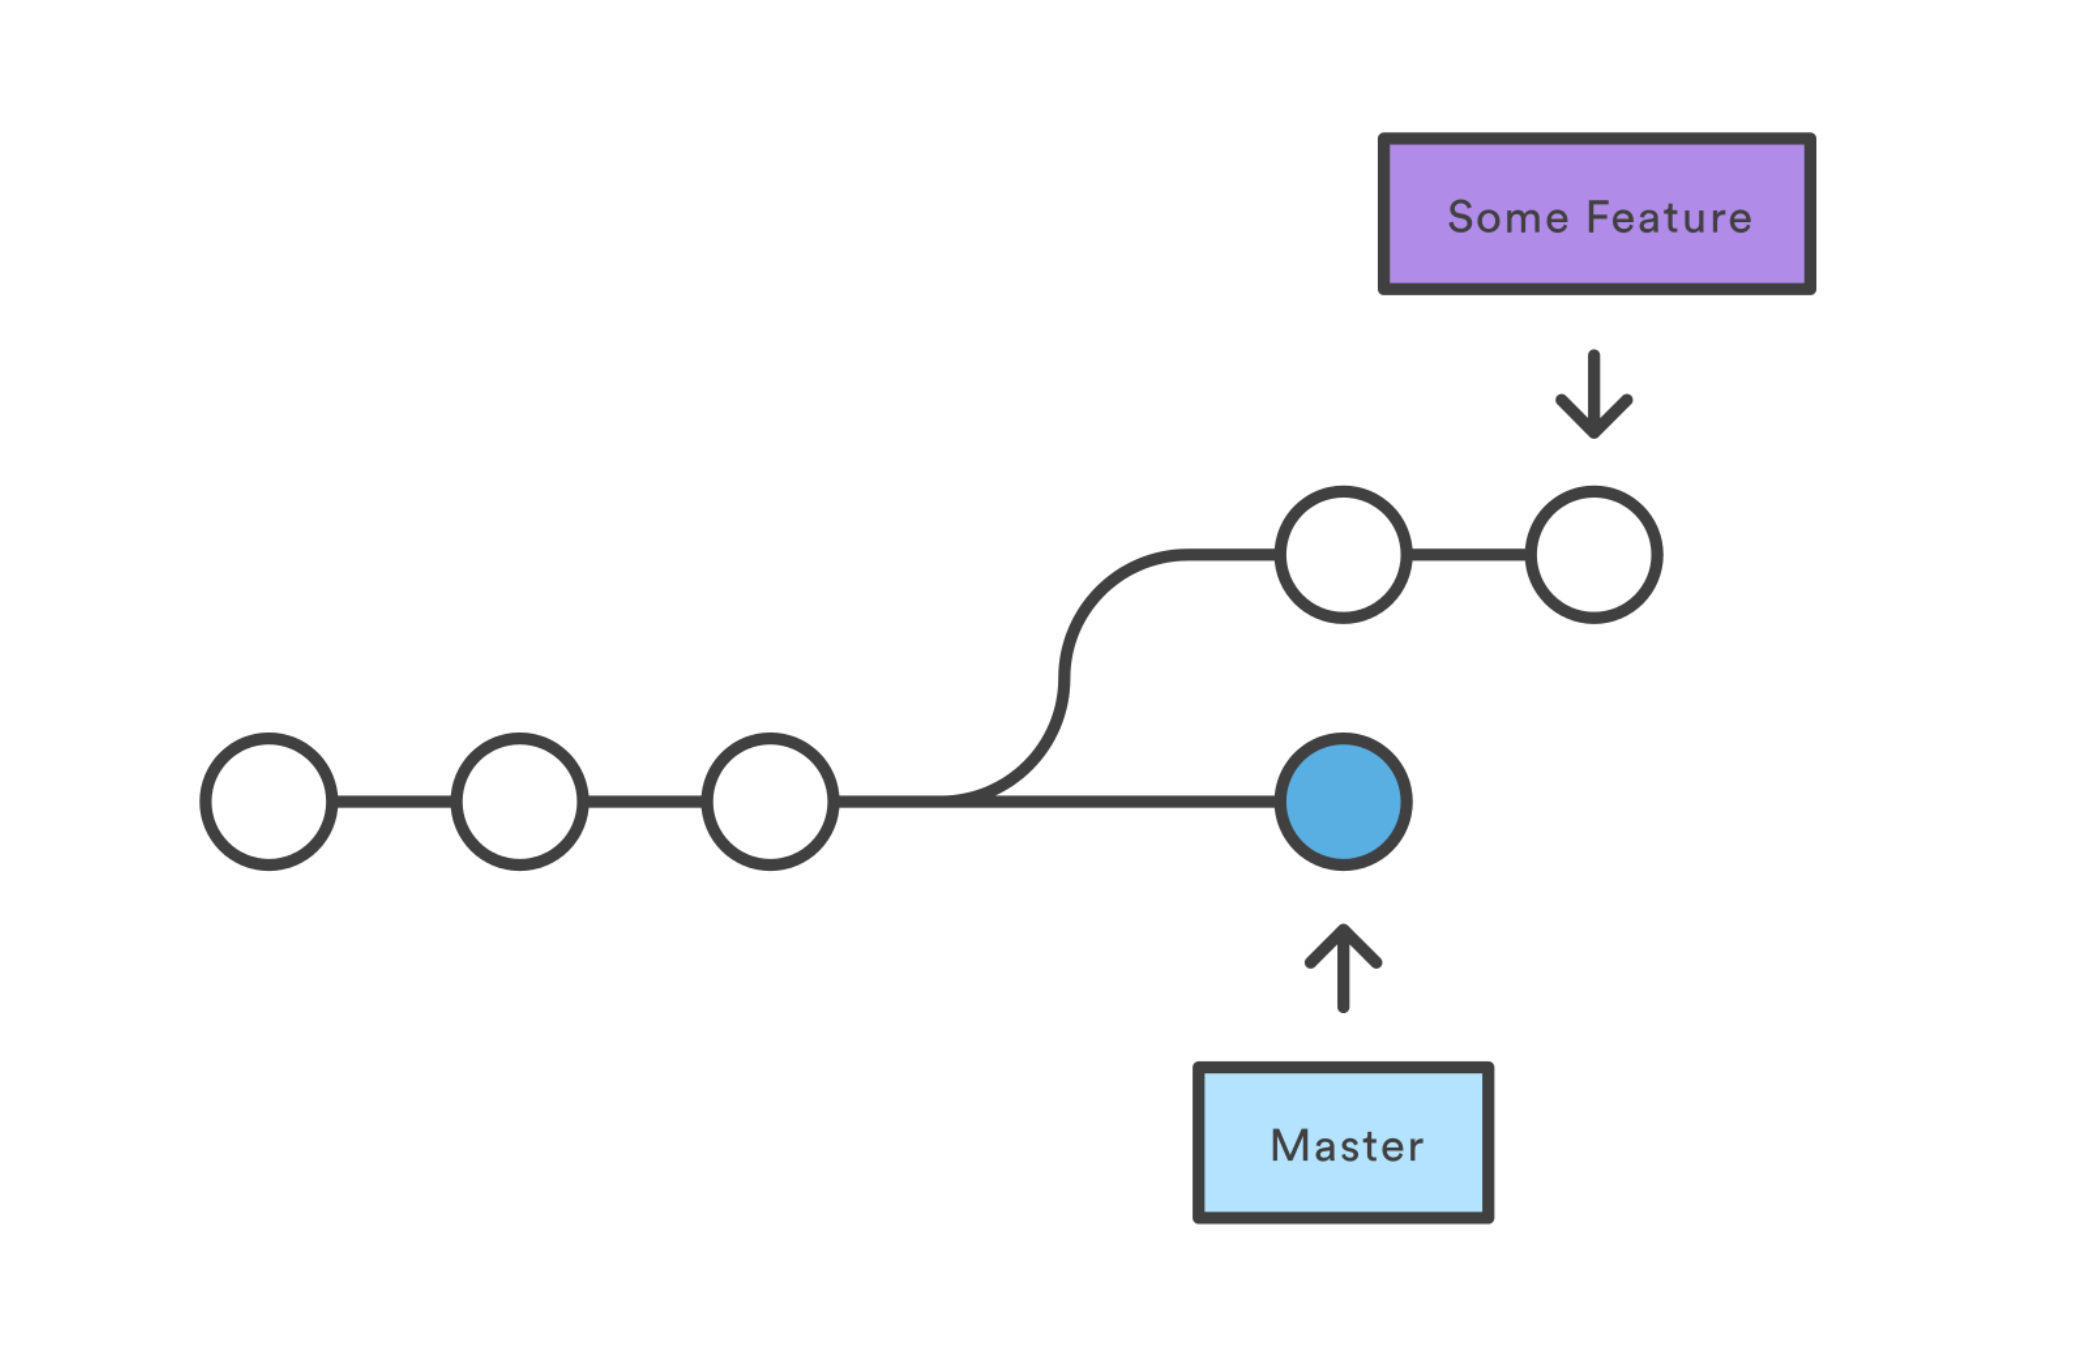
\includegraphics[scale=0.8]{figures/f15.png}\hspace{1.5cm}
\end{figure}

\end{frame}

\begin{frame}
\frametitle{Merging branches (3-way merge)}

\begin{figure}
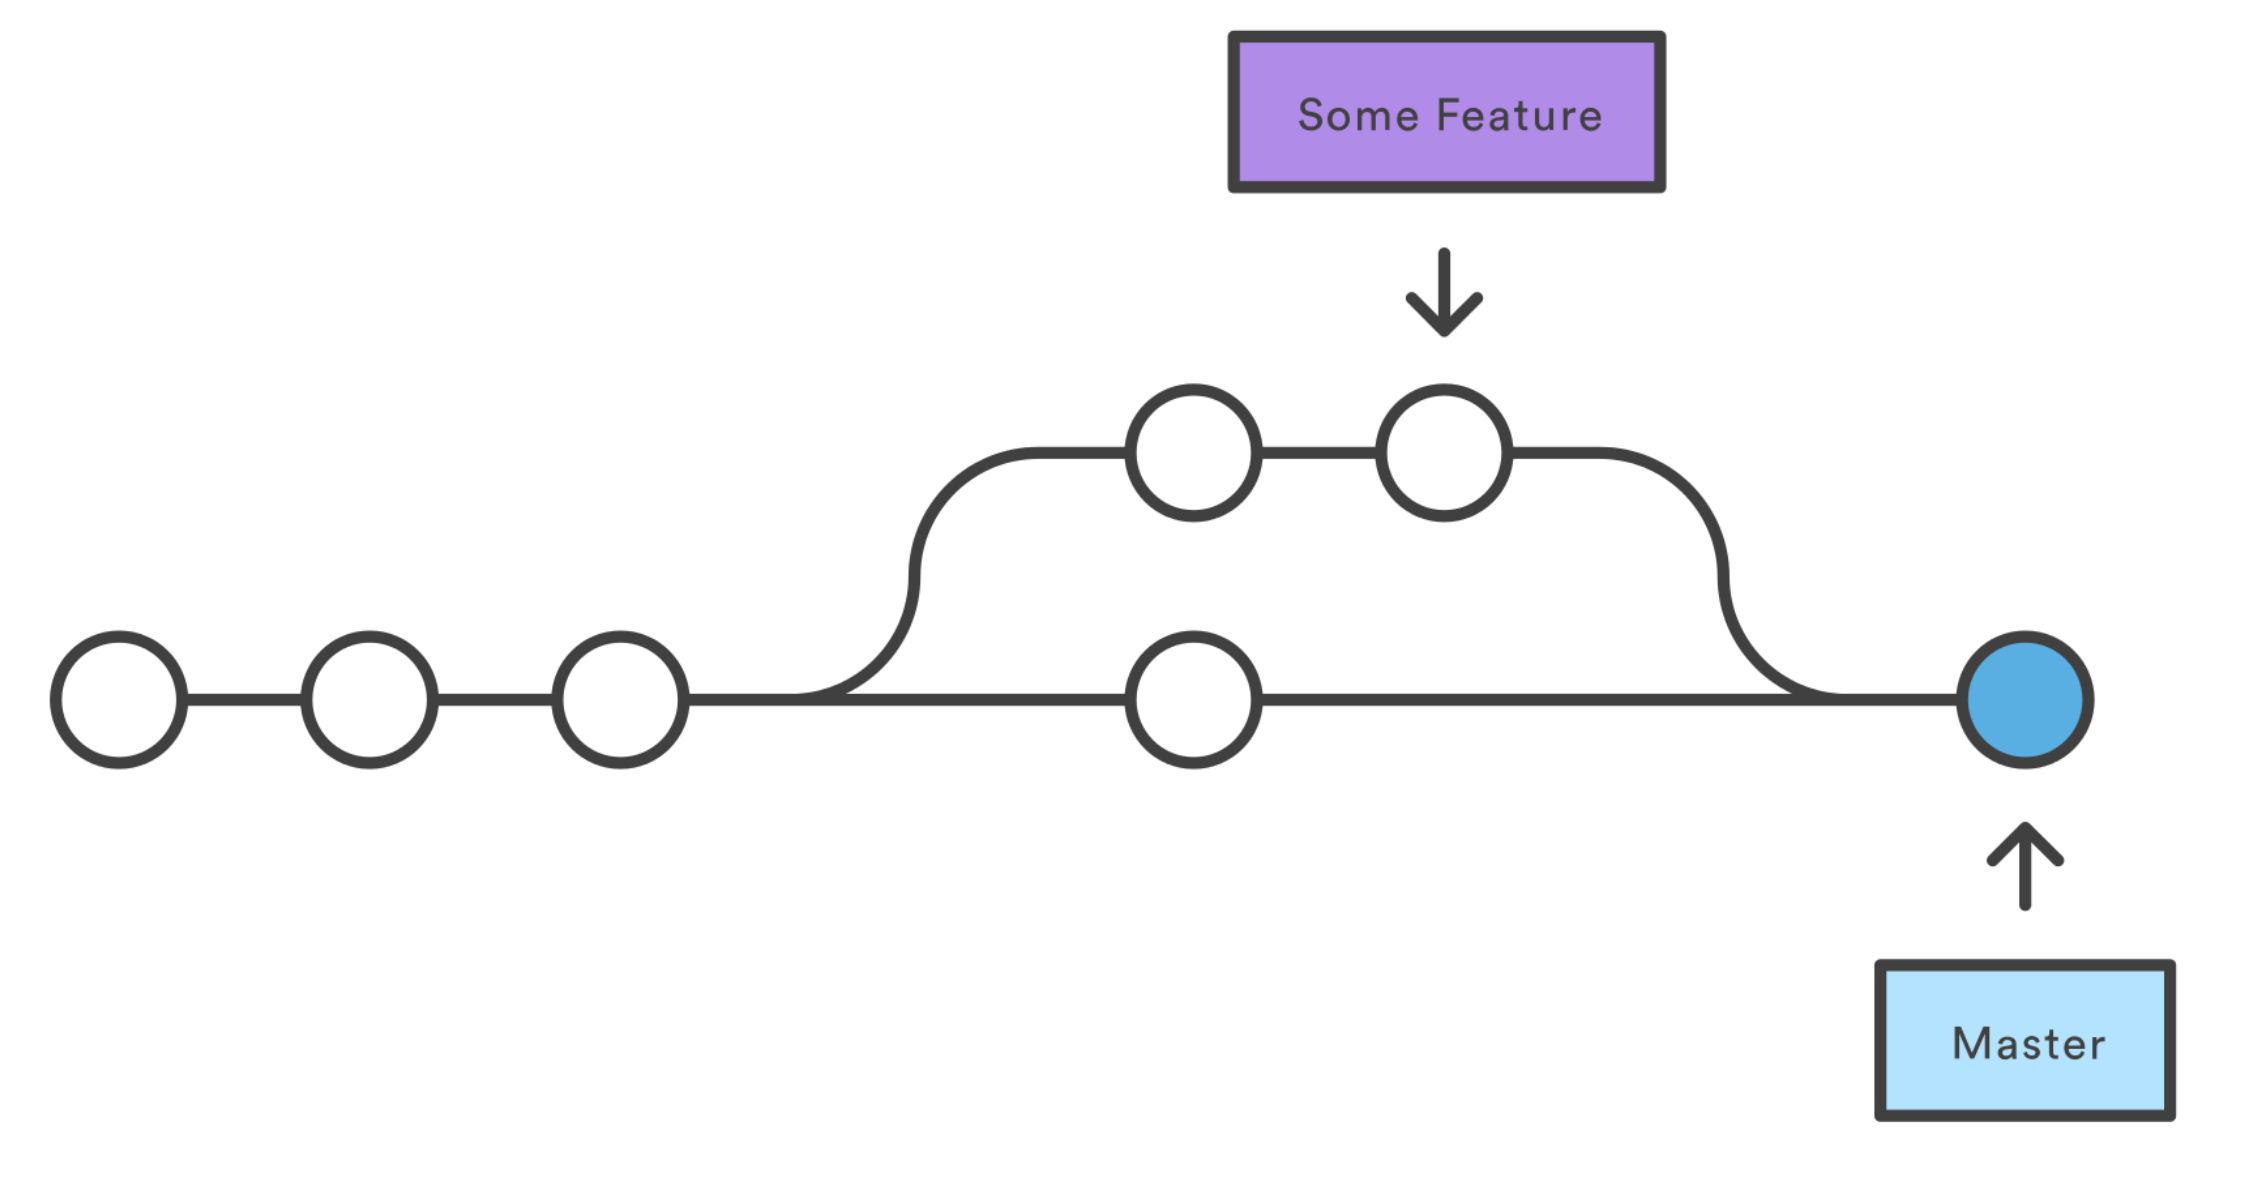
\includegraphics[scale=0.8]{figures/f16.png}
\end{figure}

\end{frame}

\begin{frame}[fragile]
\frametitle{git merge (fast-forward)}

Performing a fast-forward merge

\begin{lstlisting}
$ git checkout master
$ git merge feature-GUI-Swing
$ git log --graph --oneline --decorate
$ 
\end{lstlisting}
\end{frame}

\begin{frame}[fragile]
\frametitle{git branch -d}

Deleting branches

\begin{lstlisting}
$ git branch -d feature-GUI-Swing
$ git log --graph --oneline --decorate
\end{lstlisting}
\end{frame}


\begin{frame}[fragile]
\frametitle{git merge (3-way)}

Performing a 3-way merge

\begin{lstlisting}
$ git checkout -b feature-random
$ # perform some commits on feature-random branch
$ git checkout master
$ # perform some commits on master branch
$ git merge feature-random
$ 
\end{lstlisting}
\end{frame}



\begin{frame}[fragile]
\frametitle{Hands on - Branching and Merging (10 mins)}

Execute these commands:

\begin{lstlisting}
$ git branch <branch name>
$ git branch
$ git checkout <branch name>
$ git branch
$ # perform some commits on <branch name>
$ git checkout master
$ # perform some commits on master
$ git merge <branch name>
\end{lstlisting}
\end{frame}

\begin{frame}
\frametitle{Auto-merge and Conflicts}

\begin{itemize}

\item Merge is just another edit-stage-commit workflow.

\item Git tries to automatically merge all files by combining them (edit
phase) adding them (stage phase) and committing them (commit phase).

\item However, If the two branches changed the same \textbf{line}
of the same \textbf{file}, Git won't be able to figure out which
line to use in the final commit. 

\item When such a situation occurs, Git stops right before the commit so that
you can resolve the conflicts manually.

\end{itemize}

\end{frame}

\begin{frame}[fragile]
\frametitle{Resolving conflicts}
\begin{lstlisting}
$ cat Main.java
public class Main{
<<<<<<<<<< HEAD
int a;
==========
int b;
>>>>>>>>>> feature-random
}
$ # edit the file
$ git add Main.java
$ git commit -m "conflict resolved"
\end{lstlisting}

\end{frame}

\begin{frame}[fragile]
\frametitle{Hands on - Conflicts (2 mins)}

Execute these commands:

\begin{lstlisting}
$ # edit the <conflicted file>
$ git add <conflicted file>
$ git commit -m "<message>"
$ git log --graph --oneline --decorate
\end{lstlisting}
\end{frame}


\begin{frame}
\LARGE	
\textbf{Using Git remotely}
\end{frame}

\begin{frame}
\frametitle{Remote repository}

\begin{figure}
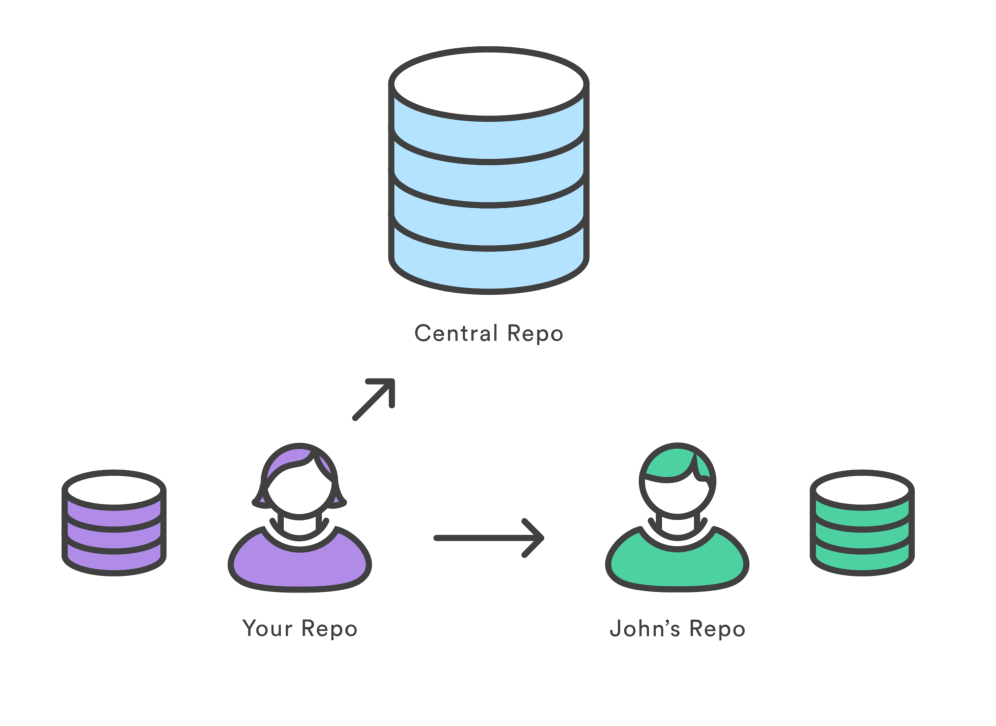
\includegraphics[scale=0.6]{figures/06.pdf}
\end{figure}

\end{frame}


\begin{frame}[fragile]
\frametitle{git remote}

The git remote command lets you create, view, and delete connections
to other repositories.

\begin{lstlisting}
$ git remote add origin https://krle@bitbucket.org/krle/test-repo.git
$ git remote
\end{lstlisting}
\end{frame}




\begin{frame}[fragile]
\frametitle{git push}
\begin{figure}

  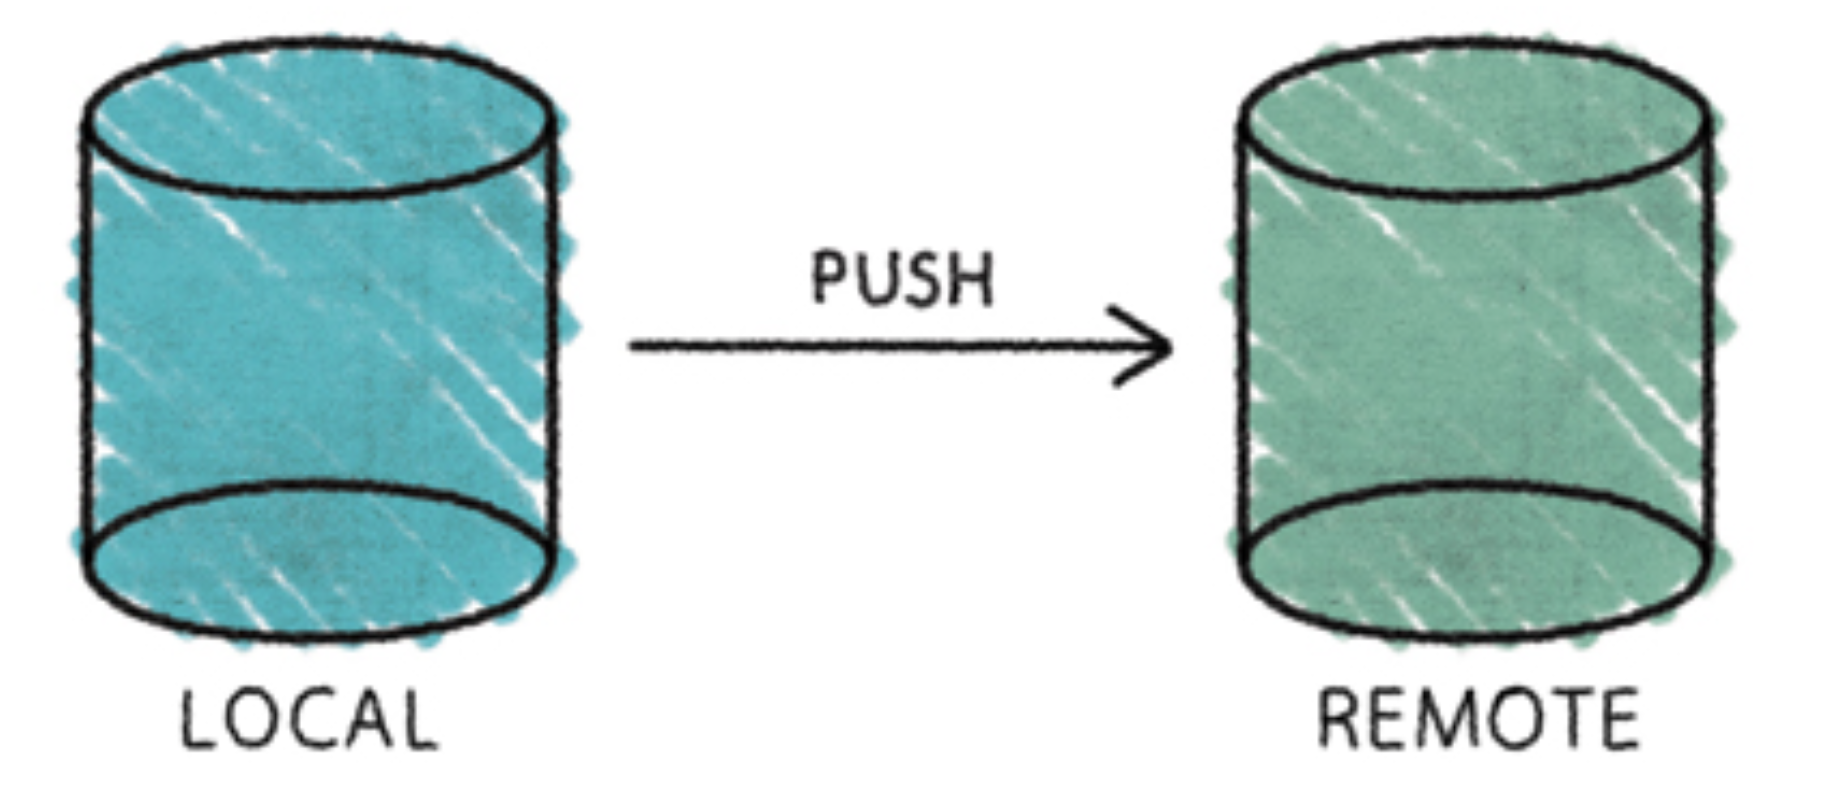
\includegraphics[scale=0.3]{figures/f6.png}
\end{figure}
\end{frame}


\begin{frame}[fragile]
\frametitle{git push}

Push command pushes the current branch to the remote repository

\begin{lstlisting}
$ git push --set-upstream origin master 
$ git branch -a
\end{lstlisting}

The \texttt{---set-upstream} or \texttt{-u} is used to bind the two
branches such that the later pull command will update the appropriate
local branch. After this you local master branch is tracking the
remote master branch.

The default behavior of push command is to push the current local
branch to its upstream remote branch (if their names match).

\texttt{git push ---all} command performs the default push behavior
for all local branches.


\end{frame}


\begin{frame}[fragile]
\frametitle{git push}

Push more branches...

\begin{lstlisting}
$ git checkout -b test
$ # make some commits to test branch
$ git push -u origin test 
$ git branch -a
$ git branch -vv
$ 
\end{lstlisting}

\texttt{git branch -vv} command shows all local branches and remote
branches that they are tracking.

\end{frame}

% \begin{frame}
% \frametitle{Configure push behavior}


% Using the configuration entry \texttt{push.default}
% you can define the action git push should take if no particular
% refspec was given. Possible values are:

% \begin{itemize}
% \item nothing - do not push anything (error out) unless a refspec is
%   explicitly given. This is primarily meant for people who want to
%   avoid mistakes by always being explicit. 

% \item current - push the current branch to update a branch with the
%   same name on the receiving end.

% \item upstream - push the current branch back to the branch whose
%   changes are usually integrated into the current branch. 

% \item simple - like upstream with an
%   added safety to refuse to push if the upstream branch's name is
%   different from the local one. When pushing to a remote that is
%   different from the remote you normally pull from, work as
%   current. 
%   \textbf{This mode has become the default in Git 2.0.}

% \item matching - push all branches having the same name on both
%   ends. 

% \end{itemize}

% \end{frame}




\begin{frame}[fragile]
\frametitle{git clone}

Finally we show how a repository can be cloned

\begin{lstlisting}
$ # use a different computer/folder
$ git clone https://krle@bitbucket.org/krle/test-repo.git
$ git branch
$ git branch -a
$ git branch -vv
$ 
\end{lstlisting}

\texttt{git clone} command fetches only the master branch from the remote
repository and sets the local master branch to track it.

\end{frame}


\begin{frame}[fragile]
\frametitle{git fetch}

Fetch command retrieves a specified remote branch.

\begin{lstlisting}
$ # stay on the second computer/folder
$ git fetch origin test
$ git branch -a
$ git branch -vv
$ git checkout -b test
$ git merge origin/test
$ git branch -vv
$ git push -u origin test
\end{lstlisting}

In order to see the fetched branch you will need a local branch to
merge with. Therefore after a fetch we create a local test branch and
merge with the remote test branch. Finally with the push command we
set the local branch to track the remote branch (without pushing any
changes).


\end{frame}


\begin{frame}[fragile]
\frametitle{git pull}
\begin{figure}

  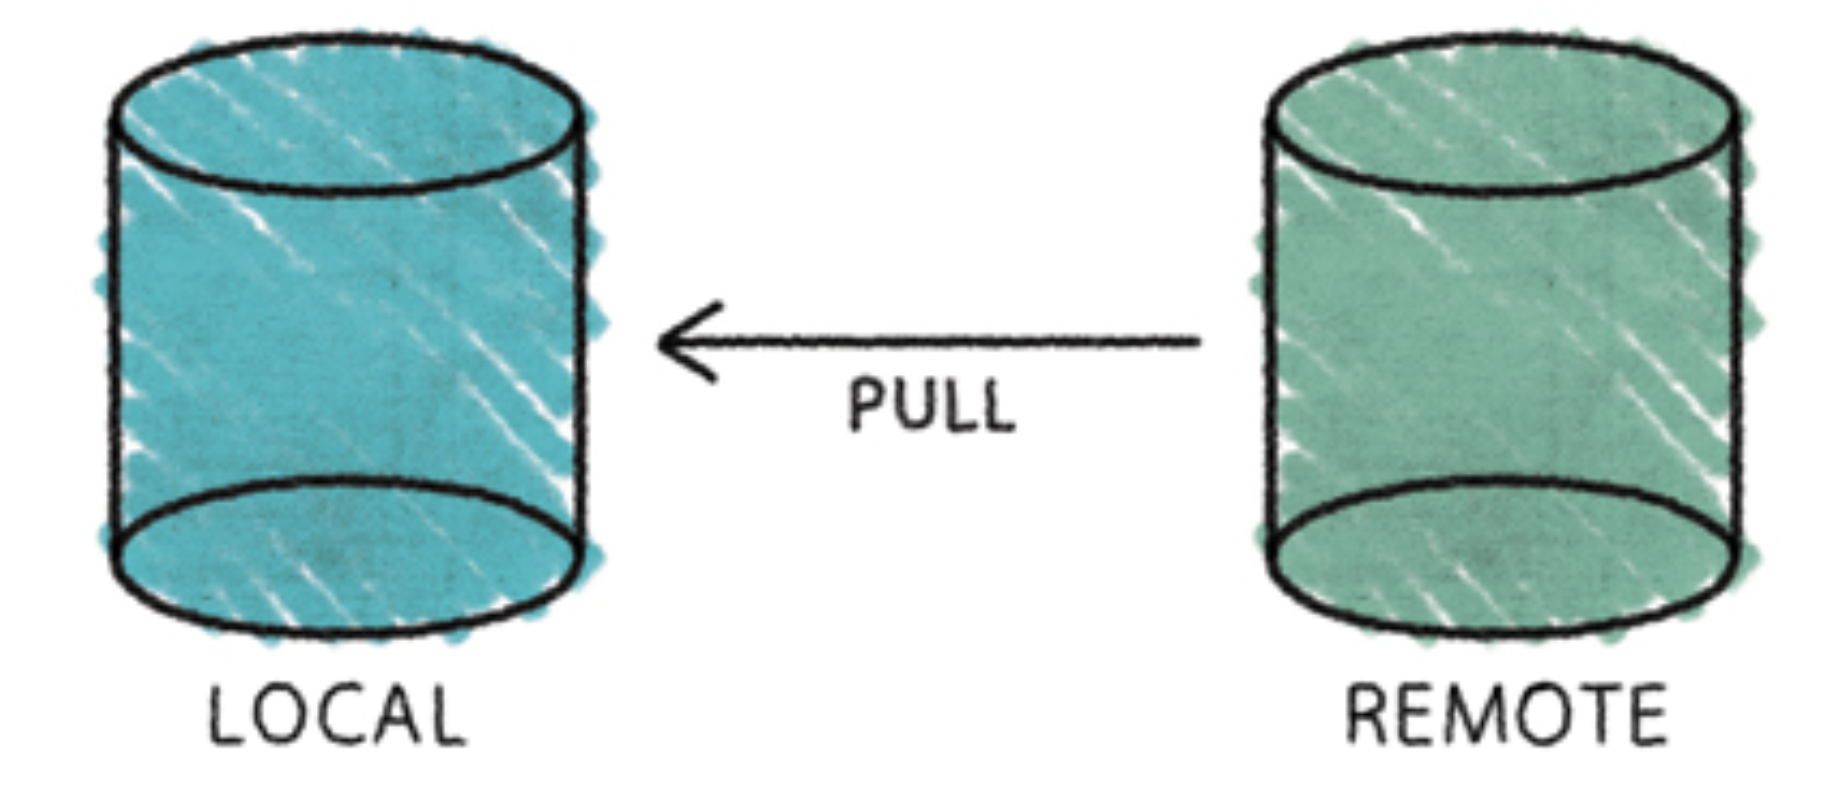
\includegraphics[scale=0.3]{figures/f7.png}
\end{figure}
\end{frame}

\begin{frame}[fragile]
\frametitle{git pull}

Pull command will perform fetching of the remote branch tracked by the
current local branch (via upstream), merge them with their
respective local branches and commit.


\begin{lstlisting}
$ # stay on the second computer/folder
$ git checkout -b some-different-branch
$ git push -u origin some-different-branch
$ git branch -vv
$ # switch to the first computer/folder
$ git pull
$ git branch -vv
$ git checkout -b some-different-branch
$ git push -u origin some-different-branch
$ git branch -vv
\end{lstlisting}

\texttt{git pull ---all} command fetches all remote branches

\end{frame}

\begin{frame}[fragile]
\frametitle{Hands on - Remote repositories (15 mins)}

Execute these commands:

\begin{lstlisting}
$ # create bitbucket test repo
$ git remote origin <URL>
$ git checkout master
$ git push -u origin master
$ 
$
\end{lstlisting}
\end{frame}


\begin{frame}
\LARGE	
\textbf{Using Git with Eclipse}
\end{frame}



\begin{frame}
\frametitle{Git references}

\begin{itemize}
\item See your guide at BEEP!
\item \url{https://git-scm.com/}
\item \url{http://gitref.org/}
\item \url{https://progit.org/}
\item \url{https://www.atlassian.com/git/}
\item Eric Sink: Version Control by Example (Chapters 1, 4, 5, 6 and
  8)
\item Tech Talk: Linus Torvalds on git
\url{https://www.youtube.com/watch?v=4XpnKHJAok8}

\end{itemize}

\end{frame}


\end{document} 

